\documentclass[preprint]{revtex4-2}

\usepackage[normalem]{ulem}
\usepackage{chemformula} % Formula subscripts using \ch{}
\usepackage[T1]{fontenc} % Use modern font encodings
\usepackage{lmodern}
\usepackage{braket}
\usepackage{physics}
\usepackage{stackengine}

\usepackage{amsmath}
\usepackage{booktabs}
\usepackage{amssymb}
\usepackage{appendix}
\usepackage{hyperref}
\usepackage{epstopdf}
\usepackage{bm}
\usepackage{dcolumn}% Align table columns on decimal point
\usepackage[version=4]{mhchem}
\DeclareMathOperator{\sgn}{sgn}
%\newcommand{\onlinecite}[1]{\hspace{-1 ex} \nocite{#1}\citenum{#1}} 
\usepackage{graphicx}
\usepackage[percent]{overpic} 
\usepackage{color}
\usepackage{transparent} 
\usepackage[shortlabels]{enumitem}
%%\usepackage{subfig} 
%\usepackage[justification=justified, format=plain, font=small, labelsep=space]{caption} %
%\usepackage[justification=justified, labelsep=space]{subcaption} 
%\captionsetup[]{labelsep=space, justification=justified}
%\DeclareCaptionLabelSeparator{none}{ }
%\usepackage{floatrow} 
%\usepackage{svg} % Include pictures in svg-format

%\newcommand{\ket}[1]{|#1\rangle}

\usepackage{setspace}
\usepackage{mathrsfs}
\usepackage{geometry}
\usepackage{braket}
\usepackage{ucs}
\usepackage{epstopdf}
\usepackage{amsfonts}
\usepackage{mathtools}
\usepackage{makeidx}
\usepackage{color}
\usepackage{bbold}
\usepackage{wrapfig}
\usepackage{comment}

\usepackage{braket}
\usepackage{mathtools}
\usepackage{appendix}
\usepackage{hyperref}
\usepackage{epstopdf}
\usepackage[version=4]{mhchem}
\usepackage[percent]{overpic} 
\usepackage{transparent} 
\usepackage{caption}
\usepackage[position=top, labelformat=parens, labelfont=bf, textfont=normalfont, singlelinecheck=off, justification=centering]{subcaption} 
\usepackage{float}


%\usepackage[caption=false]{subfig}
%\captionsetup[subfigure]{position=top, labelformat=parens, labelfont=bf,textfont=normalfont,singlelinecheck=off,justification=raggedright}

\newcommand\barbelow[1]{\stackunder[1.2pt]{$#1$}{\rule{.8ex}{.075ex}}}
\let\originalvec\vec
\renewcommand\vec[1]{\originalvec{\kern0pt #1}}
\newcommand*\pvec[1]{\vec{#1}\mkern2mu\vphantom{#1}}

\begin{document} 

\title{Cavity Polaritronics}
	%
	\author{Yannic Joshua Banthien$^{1}$}
	\affiliation{
	       $^1$Universität Hamburg\\}
	
\maketitle

\centerline{(\today)}

These notes serve to document the developements of the masters thesis of Yannic Joshua Banthien written
in 2024 and 2025.

\section{Introduction}

We want to consider the dynamics of $N$ identical doublet-doublet systems, each coupled to a single 
cavity mode, which in turn is coupled to a bath of harmonic oscillators. For this model, the full
Hamiltonian is given by 

\begin{equation}
    \mathbf{H} = \sum_{j=1}^{N} \mathbf{H}_{\text{DW,j}} + \mathbf{H}_{\text{C,int}} + \mathbf{H}_{\text{B,int}},
\end{equation}

where

\begin{equation}
    \mathbf{H}_{\text{DW,j}} = \frac{\mathbf{p}^2_j}{2\mathcal{M}} + \frac{\mathcal{M}^2\omega_0^4}{64\Delta U}\mathbf{q}_j^4
    - \frac{\mathcal{M}\omega_0^2}{4}\mathbf{q}_j^2 - \mathbf{q}_j\varepsilon,
\end{equation}

with

\begin{equation}
    \mathbf{H}_{\text{C,int}} = \frac{\mathbf{p}_y^2}{2M} + \frac{1}{2}M\Omega^2\mathbf{y}^2 + \sum_{j=1}^{N}gM\Omega^2\mathbf{y}\mathbf{q}_j,
\end{equation}

and

\begin{equation}
    \mathbf{H}_{\text{B,int}} = \sum_{\alpha} \left[ \frac{\mathbf{p}_\alpha^2}{2m_\alpha} 
    + \frac{1}{2}m_\alpha \omega_\alpha^2 \left\{ \mathbf{x}_\alpha + \frac{c_\alpha}{m_\alpha \omega_\alpha^2}
    \mathbf{y} \right\}^2 \right].
\end{equation}

Here, $\mathbf{y}$ denotes the coordinate of the cavity mode and the $\mathbf{x_\alpha}$ are the 
coordinates of the bath oscillators. 


\section{The doublet-doublet system}

We first turn to the single, bare double-well system governed by the Hamiltonian 

\begin{equation}
    \mathbf{H}_{\text{DW}} = \frac{\mathbf{p}^2}{2\mathcal{M}} + \frac{\mathcal{M}^2\omega_0^4}{64\Delta U}\mathbf{q}^4
    - \frac{\mathcal{M}\omega_0^2}{4}\mathbf{q}^2 - \mathbf{q}\varepsilon,
\end{equation}

where $\Delta U $ is the barrier height and $\varepsilon$ is the bias of the double-well.
Further, we will introduce dimensionless quantities via

\begin{equation}
\def\arraystretch{1.5}
\begin{array}{c c c}
    \tilde{t}=\omega_0t, 
    & \tilde{\mathbf{q}}=\sqrt{\mathcal{M}\omega_0/\hbar}\mathbf{q}, 
    & \tilde{\mathbf{p}}=\sqrt{1/\mathcal{M}\hbar\omega_0}\mathbf{p}, \\
    E_{\text{B}}=\Delta U/\omega_0,
    & \tilde{\varepsilon}=\sqrt{1/\mathcal{M}\hbar\omega_0^3}\varepsilon,
    & \tilde{\mathbf{H}}_{\text{DW}}=1/\hbar\omega_0\mathbf{H}_{\text{DW}}. \\
\end{array}
\end{equation}

The dimensionless Hamiltonian in units of $\hbar\omega_0$, omitting the tildes, now reads

\begin{equation}
    \mathbf{H}_{\text{DW}} = \frac{1}{2}\mathbf{p}^2+\frac{1}{64E_{\text{B}}}\mathbf{q}^4-\frac{1}{4}\mathbf{q}^2 -\mathbf{q}\varepsilon.
\end{equation}

For the sake of brevity, we set $\varepsilon=0$ in the following discussion.
Diagonalization of $\mathbf{H}_{\text{DW}}$ results in a set of energy eigenvalues and 
eigenstates 

\begin{equation}
    \left\{ \mathcal{E}_j, \ket{j} \right\}_{j\in J},
\end{equation}

with $J=\left\{ 1, 2, 3, ... \right\}$. As we are interested in the dynamics of the lowest doublet-doublet
pair, we pick our basis to be the states $\left\{ \ket{1},\ket{2},\ket{3},\ket{4} \right\}$. From this, 
we build the so-called localized basis defined as

\begin{equation}
\def\arraystretch{1.5}
\begin{array}{c c}
    \ket{L_1}=1/\sqrt{2} \left(\ket{1}-\ket{2}\right),
    & \ket{L_2}=1/\sqrt{2} \left(\ket{1}+\ket{2}\right)\\
    \ket{R_1}=1/\sqrt{2} \left(\ket{3}-\ket{4}\right),
    & \ket{R_2}=1/\sqrt{2} \left(\ket{3}+\ket{4}\right). \\
\end{array}
\end{equation}

Using these relations, it is easy to calculate the Hamiltonian of the isolated doublet-doublet system 
in the localized basis,

\begin{equation}
    \mathbf{H}^{\text{loc}}_{\text{DDS}} = \sum_{i=1,2} \left[ \bar{\mathcal{E}}_i \left( 
    \ket{L_i}\bra{L_i}+\ket{R_i}\bra{R_i} \right)- 
    \frac{\Delta_i}{2}\left( \ket{L_i}\bra{R_i}+\ket{R_i}\bra{L_i} \right) \right], 
\end{equation}

with the mean intra-doublet energies $\bar{\mathcal{E}}_1=(\mathcal{E}_1+\mathcal{E}_2)/2$, $\bar{\mathcal{E}}_2=(\mathcal{E}_3+\mathcal{E}_4)/2$
and intra-doublet energy gaps $\Delta_1=\mathcal{E}_2-\mathcal{E}_1$, $\Delta_1=\mathcal{E}_4-\mathcal{E}_3$.
Similary, the position operator in the localized can be calculated to be

\begin{equation}\label{position_operator_localized_basis}
\begin{split}
    \mathbf{q}^{\text{loc}} &= \sum_{i=1,2} q_i \left( \ket{R_i}\bra{R_i}- \ket{L_i}\bra{L_i} \right) \\
    &+ \bar{q} \left( \ket{L_1}\bra{L_2}+\ket{L_2}\bra{L_1}+\ket{R_1}\bra{R_2}+\ket{R_2}\bra{R_1} \right) \\
    &+ \frac{\Delta q}{2} \left( \ket{L_1}\bra{R_2}+\ket{R_2}\bra{L_1}-\ket{R_1}\bra{L_2}-\ket{L_2}\bra{R_1} \right),
\end{split}
\end{equation}

where $q_1 = \bra{1}\mathbf{q}\ket{2}$, $q_2 = \bra{3}\mathbf{q}\ket{4}$, 
$\bar{q}=(\bra{1}\mathbf{q}\ket{4}+\bra{2}\mathbf{q}\ket{3})/2$ and \\
$\Delta q=\bra{1}\mathbf{q}\ket{4}-\bra{2}\mathbf{q}\ket{3}$. 

Since we are after the position eigenvalues, we next diagonalize the matrix (\ref{position_operator_localized_basis}).
Analytically, this is not possible for the full expression. But, using $\Delta q/2 \ll q_i,\bar{q}$ and
noticing that (\ref{position_operator_localized_basis}) is symmetric, we can make the approximation that
$\Delta q/2 =0$, which allow us to continue the analytical calculation.
Carrying out the usual diagonalization process, the eigenstates 

\begin{equation}\label{DVR_BASIS_DEFINITION}
\def\arraystretch{1.5}
\begin{array}{c c}
    \ket{\alpha_1}=v\left(\ket{L_1}-u\ket{L_2}\right),
    & \ket{\beta_1}=v\left(\ket{R_1}+u\ket{R_2}\right)\\
    \ket{\alpha_2}=v\left(u\ket{L_1}+\ket{L_2}\right),
    & \ket{\beta_2}=v\left(u\ket{R_1}+\ket{R_2}\right) \\
\end{array}
\end{equation}

are calculated, with $v=1/\sqrt{1+u^2}$, $u=(q_1+q_{\alpha_1})/\bar{q}=-(q_2+q_{\alpha_2})/\bar{q}$ and
$q_{\alpha_i}=-q_{\beta_i}$. The $q_{\alpha_i}$ and $q_{\beta_i}$ are the position eigenvalues 
of the position eigenstates localized in the left and respectively right hand side of the double-well,
given by 

\begin{equation}\label{DDS_POSITION_EIGENVALUES}
    q_{\alpha_{1,2}} = \left[ (q_1+q_2) \mp \sqrt{(q_1-q_2)^2 + 4\bar{q}^2} \right]/2.
\end{equation}

Transforming to the DVR-basis defined by (\ref{DVR_BASIS_DEFINITION}) then finally yields the 
Hamiltonian in the DVR-basis,

\begin{equation}\label{DDS_HAMILTONIAN_DVR_BASIS}
\begin{split}
    \mathbf{H}_{\text{DDS}}^{\text{DVR}} = &- \sum_{i,j=1,2}\frac{\Delta_{\alpha_i\beta_j}}{2}(\ket{\alpha_i}\bra{\beta_j}+\ket{\beta_j}\bra{\alpha_i}) \\
    &+ \sum_{i=1,2}(E_{\alpha_i}\ket{\alpha_i}\bra{\alpha_i}+E_{\beta_i}\ket{\beta_i}\bra{\beta_i}) \\
    &- \frac{\Delta_R}{2}(\ket{\alpha_1}\bra{\alpha_2}+\ket{\alpha_2}\bra{\alpha_1}+\ket{\beta_1}\bra{\beta_2}+\ket{\beta_2}\bra{\beta_1}).
\end{split}
\end{equation}

The off-diagonal matrix elements are then 

\begin{equation}
\begin{split}
    \Delta_{\alpha_1\beta_1} &= v^2(\Delta_1+u^2\Delta_2) \\
    \Delta_{\alpha_2\beta_2} &= v^2(u^2\Delta_1+\Delta_2) \\
    \Delta_{\alpha_1\beta_2} &= \Delta_{\alpha_2\beta_1} = uv^2(\Delta_1-\Delta_2) \\
    \Delta_R &= uv^2\bar{\omega}_0, 
\end{split}
\end{equation}

where $\bar{\omega}_0=\bar{\mathcal{E}}_2-\bar{\mathcal{E}}_1$. The matrix elements of the 
Hamiltonian in the DVR-representation given by (\ref{DDS_HAMILTONIAN_DVR_BASIS}) together with
the position eigenvalues as in (\ref{DDS_POSITION_EIGENVALUES}) are the data needed to continue our
analysis. In Fig.\ref{DDS_PLOTS}, the wavefunctions of the four states is depicted in different 
representations.

\begin{figure}[H]
    \centering
    \begin{subfigure}[b]{0.45\textwidth}
        \caption{energy representation}
        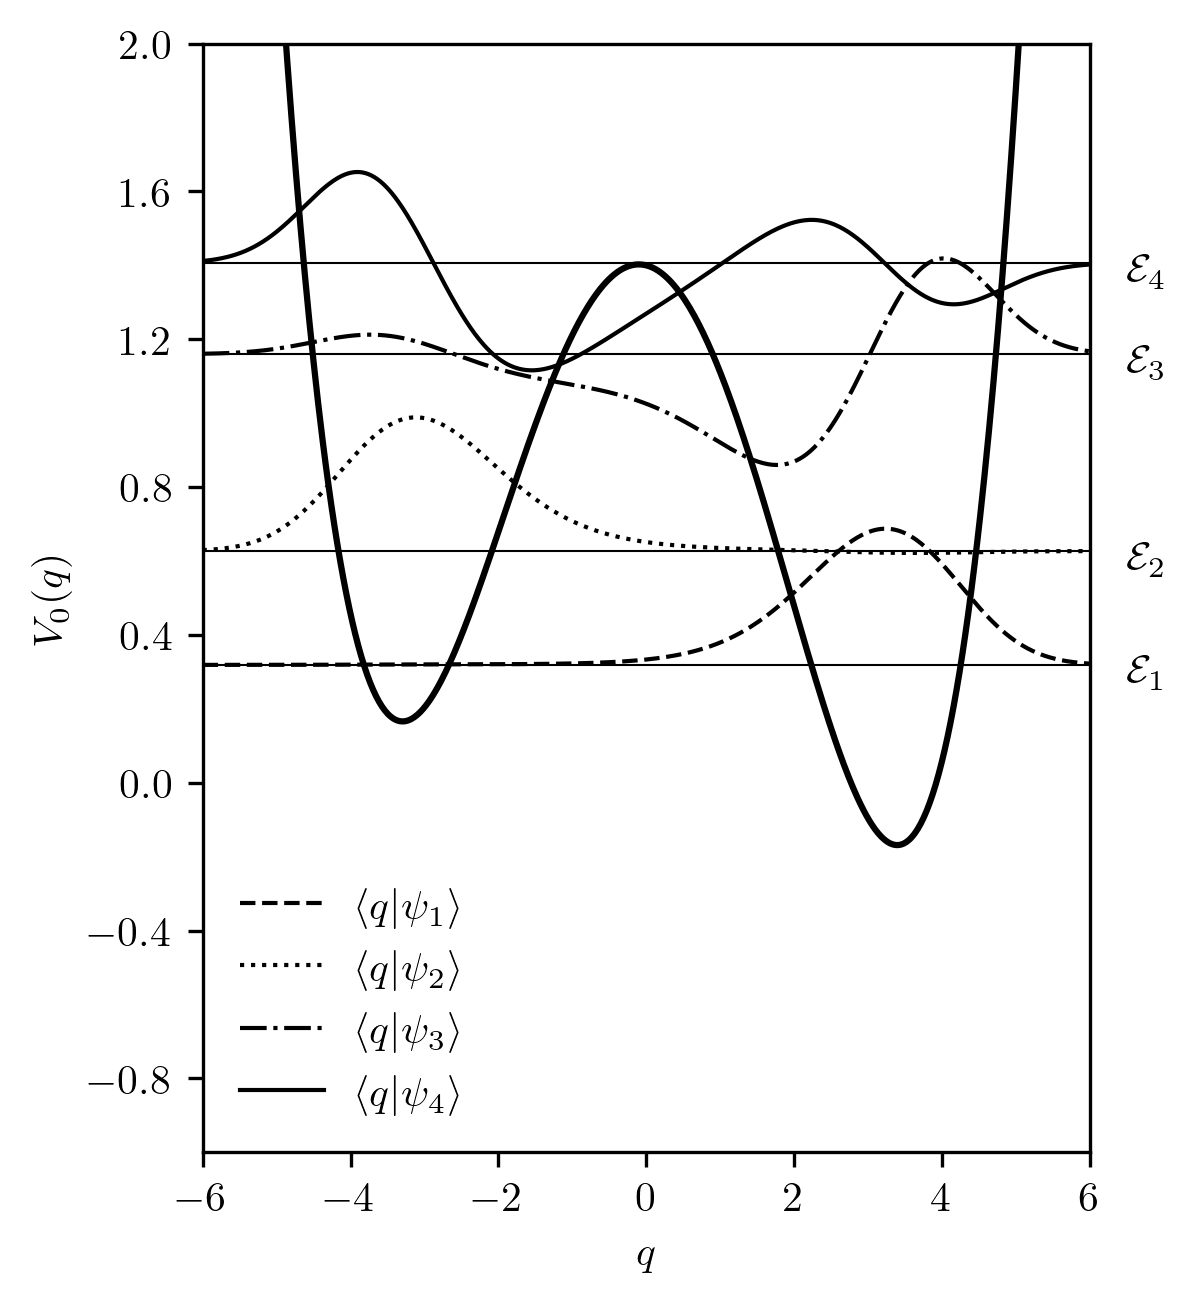
\includegraphics[width=\textwidth]{images/DDS_ENERGY_BASIS.png}
    \end{subfigure}
    \begin{subfigure}[b]{0.45\textwidth}
        \caption{localized representation}
        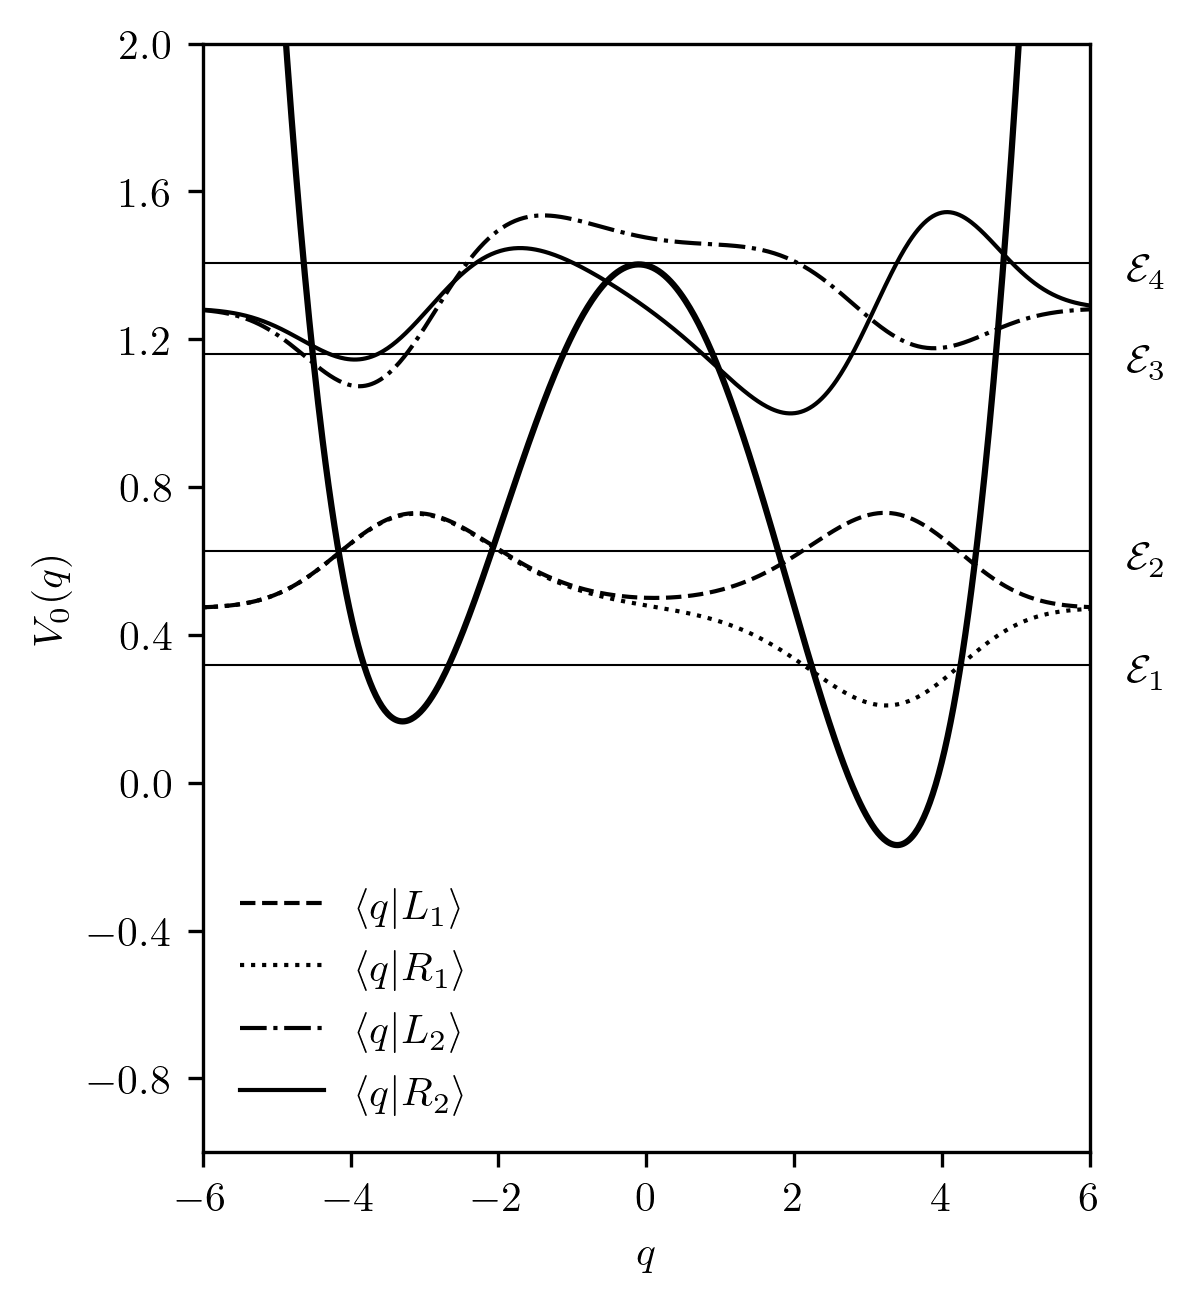
\includegraphics[width=\textwidth]{images/DDS_LOCALIZED_BASIS.png}
    \end{subfigure}
    \begin{subfigure}[b]{0.45\textwidth}
        \caption{DVR representation}
        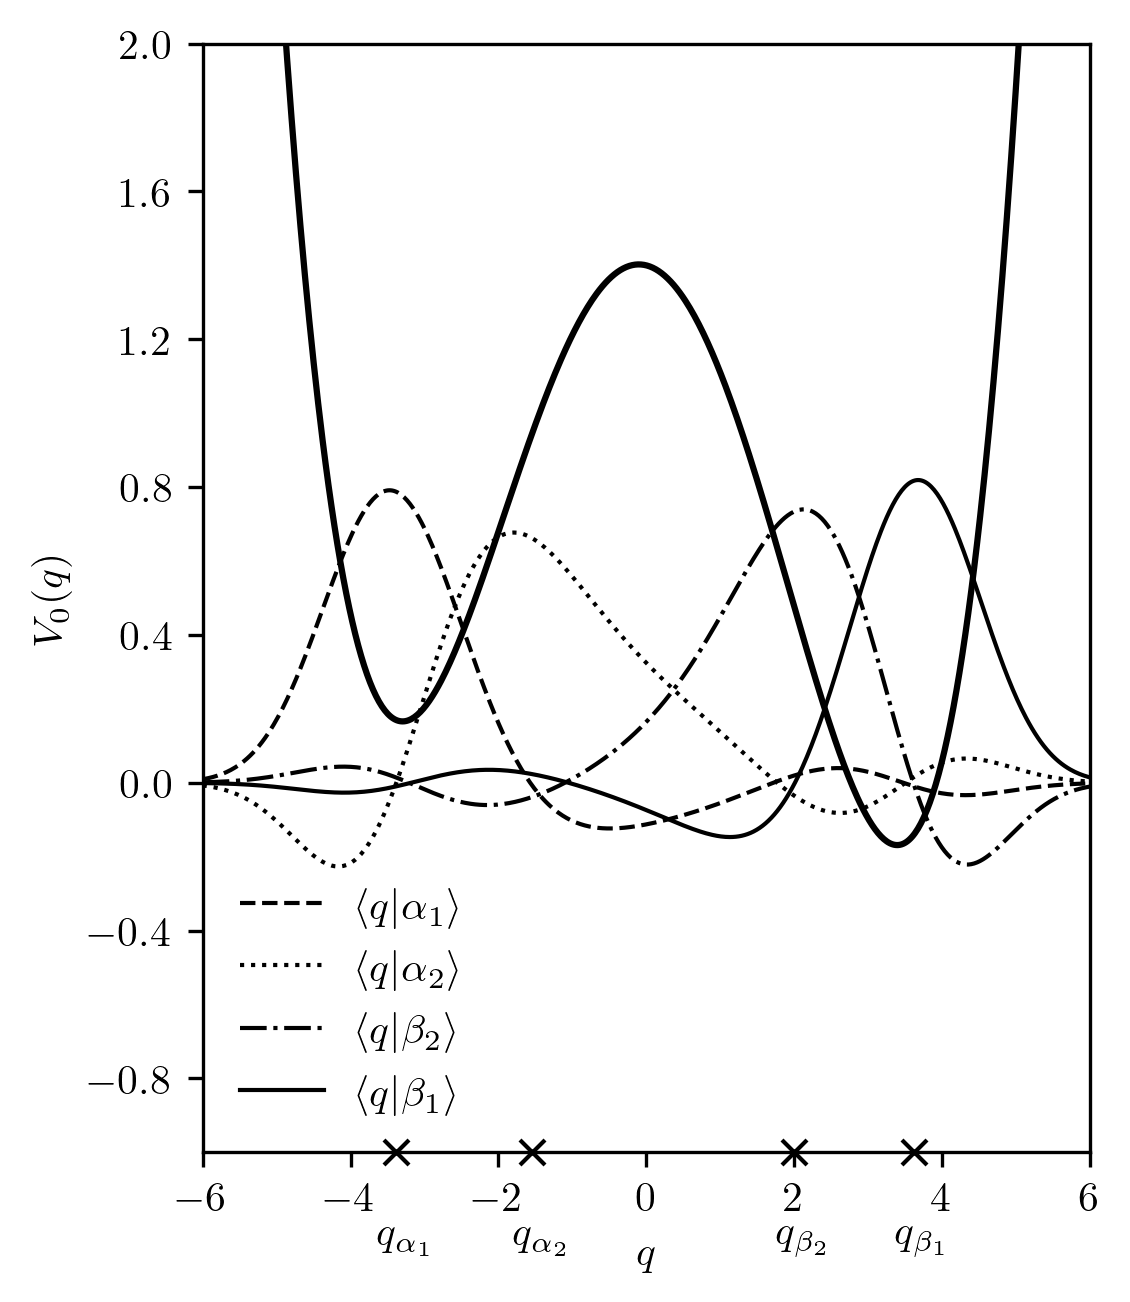
\includegraphics[width=\textwidth]{images/DDS_DVR_BASIS.png}
    \end{subfigure}
    \caption{The first four states in the (a) energy basis, (b) localized basis and (c) DVR basis.
            Here, a barrier height of $E_b=1.4$ and a bias of $\varepsilon=0.05$ are chosen.}
    \label{DDS_PLOTS}
\end{figure}

\newpage

\section{The Bath correlation function}

Next, we calculate the bath correlation function, defined by 

\begin{equation}\label{DEFINITION_BATH_CORRELATION_FUNCTION}
    Q(t)=S(t)+\text{i}R(t)=\frac{1}{\pi}\int_{0}^{\infty}\text{d}\omega\frac{J(\omega)}{\omega^2}
    \left\{\coth\frac{\omega}{2T}(1-\cos\omega t)+\text{i}\sin\omega t\right\}.
\end{equation}

The effective bath spectral density considered for our purposes will be given by

\begin{equation}\label{EFFECTIVE_BATH_SPECTRAL_DENSITY}
    J_{\text{eff}}(\omega)=\frac{2\alpha\Omega^4\omega}{(\Omega^2-\omega^2)^2+(\Gamma\omega)^2},
\end{equation}

a Lorentzian spectral density peaked at $\Omega$ and width $\Gamma$. For clarity, we start with
evaluating the real part of (\ref{DEFINITION_BATH_CORRELATION_FUNCTION}) and rewrite

\begin{equation}\label{EFFECTIVE_BATH_SPECTRAL_DENSITY_REAL_PART}
\begin{split}
    S(t)&=\frac{2\alpha\Omega^4}{\pi}\int_{0}^{\infty}\text{d}\omega\frac{1}{\omega}\frac{1}{(\Omega^2-\omega^2)^2+(\Gamma\omega)^2}
    \coth\frac{\omega}{2T}(1-\cos\omega t) \\
    &= \frac{\alpha\Omega^4}{\pi}\int_{-\infty}^{+\infty}\text{d}\omega\frac{1}{\omega}\frac{1}{(\Omega^2-\omega^2)^2+(\Gamma\omega)^2}\coth\frac{\omega}{2T}(1-\exp\text{i}\omega t).
\end{split}
\end{equation}

We can evaluate this integral using the residue theorem. To this end, we identify the poles of the first two
factors to be $\omega=0$ and $\omega=\omega_i$, $i=1,2,3,4$, where

\begin{equation}
    \def\arraystretch{1.5}
    \begin{array}{c c}
        \omega_1=\bar{\Omega}+\text{i}\Gamma/2,
        & \omega_2=-\bar{\Omega}+\text{i}\Gamma/2 \\
        \omega_3=-\bar{\Omega}-\text{i}\Gamma/2,
        & \omega_4=\bar{\Omega}-\text{i}\Gamma/2 \\
\end{array}
\end{equation}

and $\bar{\Omega}=\sqrt{\Omega^2-\Gamma^2/4}$. Further, the poles of the cotangent hyperbolicus are

\begin{equation}
    \frac{\omega}{2T} \Leftrightarrow \omega=\text{i}2\pi Tn=\text{i}\nu_n, \ n\in\mathbb{Z},
\end{equation}

with the $\nu_n$ being the familiar Matsubara frequencies. The integration contour of choice will be a half
annulus bounded by circles of radius $r$ and $R$, centered at the origin. Then, the limits $r\rightarrow0$
and $R\rightarrow\infty$ are taken, returning the sought for integral.

\begin{figure}[H]
    \centering
    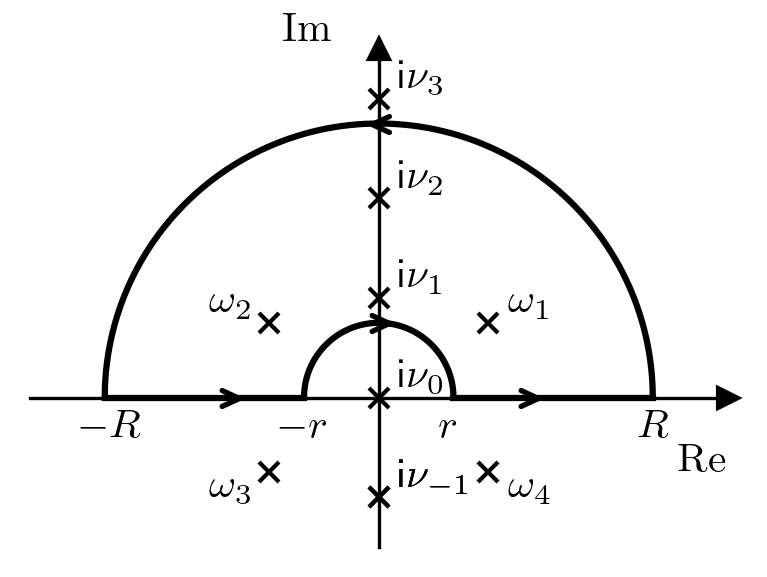
\includegraphics[width=0.5\textwidth]{images/BATH_CORRELATION_FUNCTION_INTEGRATION_CONTOUR.png}
    \caption{Integration contour used to evaluate the integral (\ref{EFFECTIVE_BATH_SPECTRAL_DENSITY_REAL_PART}).}
    \label{BATH_CORRELATION_FUNCTION_INTEGRATION_CONTOUR}
\end{figure}

Carrying out the calculation then finally gives 

\begin{equation}
    S(t)=Xt+L(e^{-(\Gamma/2)t}\cos\bar{\Omega}t-1)+Ze^{-(\Gamma/2)t}\sin\bar{\Omega}t+S_{\text{Mats}}(t),
\end{equation}

where 

\begin{align}
    X &= 2\alpha T \\
    L &= \frac{\alpha}{\Gamma\bar{\Omega}}\frac{(\Gamma^2/4-\bar{\Omega}^2)\sinh\bar{\Omega}/T
            +\Gamma\bar{\Omega}\sin\Gamma/(2T)}{\cosh\bar{\Omega}/T-\cos\Gamma/(2T)} \\
    Z &= \frac{\alpha}{\Gamma\bar{\Omega}}\frac{-\Gamma\bar{\Omega}\sinh\bar{\Omega}/T
    +(\Gamma^2/4-\bar{\Omega}^2)\sin\Gamma/(2T)}{\cosh\bar{\Omega}/T-\cos\Gamma/(2T)}.
\end{align}

The last term $S_{\text{Mats}}(t)$ is a function of the Matsubara frequencies, 

\begin{equation}
    S_{\text{Mats}}(t)=-4\alpha\Omega^4T\sum_{n=1}^{\infty}
    \frac{1}{(\Omega^2+\nu_n^2)^2-\Gamma^2\nu_n^2} \Big( \frac{\exp(-\nu_n t)-1}{\nu_n} \Big).
\end{equation}

In the regime of $T>\Gamma/(2\pi)$, this term can be neglected, as we will.
An analogous calculation for the imaginary part of (\ref{DEFINITION_BATH_CORRELATION_FUNCTION}) yields 

\begin{equation}
    R(t) = \alpha - \alpha e^{-(\Gamma/2)t}(N\sin\bar{\Omega}t+\cos\bar{\Omega}t),
\end{equation}

where $N=(\Gamma^2/4-\bar{\Omega}^2)/(\Gamma\bar{\Omega})$.
In order to derive an analytical expression for the rate matrix elements, we will employ the so-called 
weak-damping approximation (WDA). Since we are interested in the case of a sharpely peaked bath spectral density,
meaning that $\kappa = \Gamma/(2\pi\Omega) \ll 1$, we may expand the bath correlation function to first order
in $\kappa$. This procedure gives the result 

\begin{align}
    S(\tau) &= Y (\cos\Omega\tau-1) + A\tau\cos\Omega\tau + B\tau + C\sin\Omega\tau + \mathcal{O}(\kappa^2) \\
    R(\tau) &= W\sin\Omega\tau + V \left( 1 - \cos\Omega\tau - \frac{\Omega}{2}\tau\sin\Omega\tau \right) + \mathcal{O}(\kappa^2),
\end{align}

with the $\kappa$-independent terms 

\begin{equation}
    Y = - \frac{4g^2}{\Omega^2}\coth\frac{\Omega}{2T}, \ \ \ W = \frac{4g^2}{\Omega^2}
\end{equation}

and the terms linear in $\kappa$

\begin{align}
    A &= -\Gamma \frac{Y}{2}, \ \ \ B = \Gamma\frac{8g^2T}{\Omega^3} \\
    C &= -\Gamma \frac{2g^2}{\Omega^3}\frac{\Omega/T+2\sinh\Omega/T}{\cosh\Omega/T}, \ \ \ V = \Gamma \frac{4g^2}{\Omega^3}.
\end{align}

\end{document}